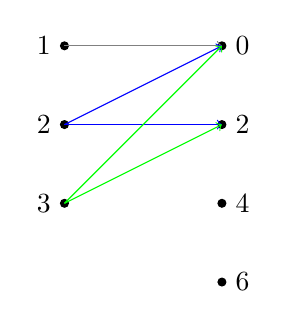
\begin{tikzpicture}
\foreach \y/\t in {0/1,-1/2,-2/3}
{
	\draw[fill=black] (0,\y) circle (0.05);
	\node at (-0.05,\y) [left] {$\t$};
}

\foreach \y/\t in {0/0,-1/2,-2/4,-3/6}
{
	\draw[fill=black] (2,\y) circle (0.05);
	\node at (2.05,\y) [right] {$\t$};
}

\draw[->,color=gray] (0,0) -- (2,0);

\draw[->,color=blue] (0,-1) -- (2,0);
\draw[->,color=blue] (0,-1) -- (2,-1);

\draw[->,color=green] (0,-2) -- (2,0);
\draw[->,color=green] (0,-2) -- (2,-1);
\end{tikzpicture}
